\section*{Phần 10.4}
\subsection*{Bài 2}
Mỗi danh sách đỉnh sau đây có lập thành một đường đi trong đồ thị dưới đây không? Những đường đi nào là đơn giản? Đâu là chu trình? Độ dài của những đường đi đó là bao nhiêu?
\begin{enumerate}[label=\alph*)]
    \item a, b, e, c, b
    \item a, d, a, d, a
    \item a, d, b, e, a
    \item a, b, e, c, b, d, a
\end{enumerate}
\begin{center}
    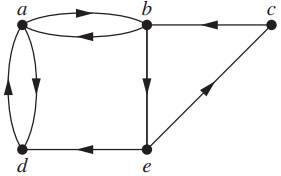
\includegraphics[scale=0.75]{10.4_2.png}
\end{center}
\begin{proof}.
    \begin{enumerate}[label=\alph*)]
        \item Kiểm tra các cặp đỉnh liên tiếp nhau đều tồn tại đường đi giữa chúng, vậy đây là một đường đi độ dài 5.
        \item Kiểm tra các cặp đỉnh liên tiếp nhau đều tồn tại đường đi giữa chúng, vậy đây là một đường đi độ dài 5.
        \item Vì không có đường đi giữa d và b nên đây không phải đường đi hợp lệ.
        \item Vì không có đường đi giữa b và d nên đây không phải đường đi hợp lệ.
    \end{enumerate}
\end{proof}
\subsection*{Bài 6}
Có bao nhiêu thành phần liên thông trong các đồ thị từ bài 3 đến bài 5? Với mỗi đồ thị hãy tìm từng thành phần liên thông.
\begin{center}
    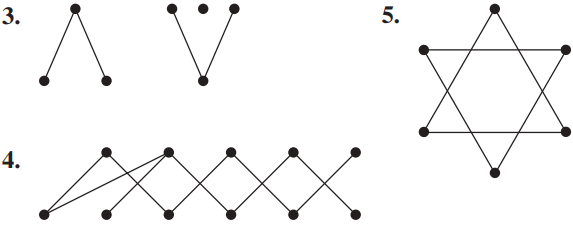
\includegraphics[scale=0.5]{10.4_6.png}
\end{center}
\begin{proof}
    Bài 3 có 3 thành phần liên thông, 1 là 3 đỉnh xếp thành hình chữ A, 2 là 3 đỉnh xếp thành hình chữ V và 3 là một đỉnh ở giữa chữ V đó, các thành phần này không có cạnh nào nối chúng với nhau. Bài 4 và 5 chỉ có một thành phần vì tất cả các đỉnh đều được nối với nhau.
\end{proof}
\subsection*{Bài 16}
